%%%%%%%%%%%%%%%%%%%%%%%%%%%%%%%%%%%%%%%%%
% Beamer Presentation
% LaTeX Template
% Version 1.0 (10/11/12)
%
% This template has been downloaded from:
% http://www.LaTeXTemplates.com
%
% License:
% CC BY-NC-SA 3.0 (http://creativecommons.org/licenses/by-nc-sa/3.0/)
%
%%%%%%%%%%%%%%%%%%%%%%%%%%%%%%%%%%%%%%%%%

%----------------------------------------------------------------------------------------
%	PACKAGES AND THEMES
%----------------------------------------------------------------------------------------

\documentclass{beamer}

\mode<presentation> {

	%\usetheme{default}
	%\usetheme{AnnArbor}
	%\usetheme{Antibes}
	%\usetheme{Bergen}
	%\usetheme{Berkeley}
	%\usetheme{Berlin}
	%\usetheme{Boadilla}
	%\usetheme{CambridgeUS}
	%\usetheme{Copenhagen}
	%\usetheme{Darmstadt}
	%\usetheme{Dresden}
	%\usetheme{Frankfurt}
	%\usetheme{Goettingen}
	%\usetheme{Hannover}
	%\usetheme{Ilmenau}
	%\usetheme{JuanLesPins}
	%\usetheme{Luebeck}
	%\usetheme{Madrid}
	%\usetheme{Malmoe}
	%\usetheme{Marburg}
	%\usetheme{Montpellier}
	%\usetheme{PaloAlto}
	\usetheme{Pittsburgh}
	%\usetheme{Rochester}
	%\usetheme{Singapore}
	%\usetheme{Szeged}
	%\usetheme{Warsaw}

	%\usecolortheme{albatross}
	\usecolortheme{beaver}
	%\usecolortheme{beetle}
	%\usecolortheme{crane}
	%\usecolortheme{dolphin}
	%\usecolortheme{dove}
	%\usecolortheme{fly}
	%\usecolortheme{lily}
	%\usecolortheme{orchid}
	%\usecolortheme{rose}
	%\usecolortheme{seagull}
	%\usecolortheme{seahorse}
	%\usecolortheme{whale}
	%\usecolortheme{wolverine}
}

\usepackage{graphicx}
\usepackage{booktabs}
\usepackage{multicol}
\usepackage{amsmath, bm}
\usepackage{fontspec}
\setsansfont{Calibri}[
    Path=Font/,
    Scale=0.9,
    Extension = .ttf,
    UprightFont=*-Regular,
    BoldFont=*-Bold,
    ItalicFont=*-Italic,
    BoldItalicFont=*-BoldItalic
    ]
\usepackage{unicode-math}
\setmathfont{Libertinus Math}

\usepackage{ragged2e}
\justifying\let\raggedright\justifying
\usepackage{tikz}
\usetikzlibrary{positioning}
\usetikzlibrary{calc}

\setbeamercolor{postit}{fg=black,bg=yellow!20}

%----------------------------------------------------------------------------------------
%	TITLE PAGE
%----------------------------------------------------------------------------------------

\title[Asset Pricing]{\textbf{Asset Pricing}}

\subtitle{4. Anomalies}

\author[Cheng Hang]{Cheng Hang}
\institute[DUFE]
{School of Fintech \\
	Dongbei University of Finance \& Economics \\
	\medskip
	\textbf{chenghangch@qq.com}
}
\date{\today}

\AtBeginSection[]
{
	\begin{frame}{Content}
		\begin{columns}[t]
			\begin{column}{0.5\textwidth}
				\tableofcontents[sections={1-3},sectionstyle=show/shaded,subsectionstyle=show/shaded/hide]
			\end{column}
			\begin{column}{0.5\textwidth}
				\tableofcontents[sections={4-6},sectionstyle=show/shaded,subsectionstyle=show/shaded/hide]
			\end{column}
		\end{columns}
		\addtocounter{framenumber}{-1}
	\end{frame}
}

%----------------------------------------------------------------------------------------
%	Begin
%----------------------------------------------------------------------------------------

\begin{document}

\begin{frame}
	\titlepage
\end{frame}

\section{Why Anomalies Matter}

\begin{frame}{From CAPM Failure to the Anomaly Literature}
	\begin{itemize}
		\item CAPM predicts a simple cross-sectional restriction: \textbf{market beta is the only priced risk}.
		\item Empirically, the Security Market Line is too flat: low-$\beta$ assets earn ``too much," and high-$\beta$ assets earn ``too little."
		\item Average returns also line up with \textbf{firm characteristics} such as size, book-to-market, past return, profitability, and investment.
		\item This launches the anomaly research program:
		\begin{enumerate}
			\item Is CAPM missing relevant sources of risk?
			\item Are prices distorted by behavioral or institutional frictions?
			\item Or are we looking at fragile in-sample patterns?
		\end{enumerate}
	\end{itemize}

	\vspace{0.4cm}
	\begin{beamercolorbox}[sep=0.5em,wd=\linewidth,rounded=true,shadow=true]{postit}
		\textbf{Key idea:} Anomaly research is the bridge from beta pricing to multi-factor asset pricing.
	\end{beamercolorbox}
\end{frame}

\begin{frame}{What Exactly Is an Anomaly?}
	An anomaly is \textbf{model-relative}. For a candidate long-short strategy $A$:
	\begin{equation}
		R_{A,t}^e = \alpha_A + \beta_A' f_t + \varepsilon_{A,t}
	\end{equation}

	\begin{itemize}
		\item If $\alpha_A \neq 0$ relative to a benchmark model, the model fails on that spread.
		\item The same strategy may be an anomaly under CAPM but not under FF3, FF5, or $q$-factor.
		\item For doctoral research, a convincing anomaly usually needs:
		\begin{enumerate}
			\item \textbf{Statistical reliability}: robust $t$-statistics under sensible specifications.
			\item \textbf{Economic magnitude}: sizable spread after standard risk adjustment.
			\item \textbf{Implementability}: not driven entirely by microcaps, illiquidity, or impossible shorts.
		\end{enumerate}
	\end{itemize}
\end{frame}

\begin{frame}{A Taxonomy of Canonical Anomalies}
	\begin{columns}[t]
		\begin{column}{0.48\textwidth}
			\textbf{Valuation / Relative Price}
			\begin{itemize}
				\item Size
				\item Book-to-market
				\item Earnings yield
				\item Cash-flow yield
			\end{itemize}

			\textbf{Price Dynamics}
			\begin{itemize}
				\item Momentum
				\item Short-term reversal
				\item Long-run reversal
			\end{itemize}
		\end{column}
		\begin{column}{0.48\textwidth}
			\textbf{Fundamentals / Production}
			\begin{itemize}
				\item Profitability
				\item Investment
				\item Accruals
				\item Issuance
			\end{itemize}

			\textbf{Frictions / Risk Proxies}
			\begin{itemize}
				\item Liquidity
				\item Low-risk / low-beta
				\item Idiosyncratic volatility
			\end{itemize}
		\end{column}
	\end{columns}

	\vspace{0.4cm}
	\textbf{Unifying question:} do these signals proxy for \textbf{state-variable risk}, \textbf{mispricing}, or \textbf{research design artifacts}?
\end{frame}

\begin{frame}{What the Big Synthesis Papers Actually Do}
	\begin{itemize}
		\item \href{https://doi.org/10.1111/j.1540-6261.2008.01371.x}{\textcolor{blue}{Fama and French (2008)}}: benchmark comparison of prominent anomalies; size, value, and momentum remain the key stress tests for factor models.
		\item \href{https://doi.org/10.1093/rfs/hhu068}{\textcolor{blue}{Hou, Xue, and Zhang (2015)}}: shows how profitability and investment logic can ``digest'' many anomalies within a production-based framework.
		\item \href{https://doi.org/10.1093/rfs/hhy131}{\textcolor{blue}{Hou, Xue, and Zhang (2020)}}: imposes a common protocol on 452 U.S. anomalies and emphasizes microcaps, multiple testing, and implementation.
		\item \href{https://doi.org/10.1093/rfs/hhaa019}{\textcolor{blue}{Karolyi and Van Nieuwerburgh (2020)}}: survey-style editorial for the RFS special issue on new methods for the cross-section, highlighting replication, ML, and SDF extraction.
	\end{itemize}

	\vspace{0.3cm}
	\begin{beamercolorbox}[sep=0.4em,wd=\linewidth,rounded=true,shadow=true]{postit}
		\textbf{Reading strategy:} first learn the classic anomalies, then learn how later papers compress, replicate, or overturn them.
	\end{beamercolorbox}
\end{frame}

\begin{frame}{China-Focused Synthesis Papers}
	\begin{itemize}
		\item \href{https://doi.org/10.1016/j.pacfin.2022.101739}{\textcolor{blue}{Han and Shi (2022)}} study \textbf{62 Chinese anomalies}: trading-friction anomalies are strongest, sentiment matters, and publication decay is weak.
		\item \href{https://doi.org/10.1287/mnsc.2023.4904}{\textcolor{blue}{Li, Liu, Liu, and Wei (2024)}} replicate \textbf{469 anomaly variables} in A-shares: \textbf{83.37\%} fail under reliable breakpoints and value-weighted tests; CH3, CH4, and $q$-factor perform best.
		\item \href{https://eng.pbcsf.tsinghua.edu.cn/dfiles/wp6.pdf}{\textcolor{blue}{Hou, Qiao, and Zhang (August 2024 draft)}} construct \textbf{454 Chinese strategies}: only 38 raw strategies survive a multiple-testing cutoff of $t=2.85$, and none survive after risk adjustment.
		\item \href{https://www.cfrn.com.cn/uploads/master/paper/20240728/66a60a40ddd07.pdf}{\textcolor{blue}{Wang and Zhu (March 2024 draft)}} compare \textbf{11 factor models} on \textbf{105 Chinese anomalies}: Q5 dominates in time-series and anomaly-explaining tests, while Q5, FF6, and IPCA5 jointly lead in cross-sectional horse races.
	\end{itemize}
\end{frame}

\begin{frame}{Anomaly Types Already Covered in This Project}
	\small
	\begin{table}
		\centering
		\resizebox{\linewidth}{!}{
			\begin{tabular}{p{2.5cm}p{5.5cm}p{3.2cm}}
				\toprule
				\textbf{Family} & \textbf{Representative Signals Already Mentioned} & \textbf{Main Lens} \\
				\midrule
				Valuation / Price ratios & Size, book-to-market, earnings yield, shell value & Risk vs. distress vs. mispricing \\
				Price dynamics & Momentum, short-term reversal, long-run reversal, factor momentum & Underreaction / overreaction \\
				Fundamentals / production & Profitability, investment, asset growth, issuance, intangibles / human capital & $q$-theory, production SDF \\
				Frictions / behavioral & Liquidity, turnover, IVOL, MAX, low-risk, sentiment, speculation & Limits to arbitrage / lottery demand \\
				China-specific institutional & A/B share clientele, short-sale constraints, retail dominance, regulation & Market structure and clientele effects \\
				\bottomrule
			\end{tabular}
		}
	\end{table}

	\normalsize
	\textbf{Interpretation:} the current project already covers \textbf{price-based}, \textbf{fundamental-based}, and \textbf{friction-based} anomaly families.
\end{frame}

\section{Research Design}

\begin{frame}{The Canonical Empirical Workflow}
	\begin{enumerate}
		\item Choose a signal $z_{i,t}$ observed at time $t$.
		\item Sort assets into portfolios by $z_{i,t}$ using NYSE or market-specific breakpoints.
		\item Hold the portfolios over $t+1$ (or over a horizon $K$) and compute the spread:
		\begin{equation}
			R^{A}_{t+1} = R_{High,t+1} - R_{Low,t+1}
		\end{equation}
		\item Test whether the spread survives benchmark adjustment:
		\begin{equation}
			R^{A}_{t+1} = \alpha_A + \beta_A' f_{t+1} + \varepsilon_{t+1}
		\end{equation}
	\end{enumerate}

	\begin{itemize}
		\item Important design choices: equal- vs. value-weighting, breakpoints, rebalancing, skip-months, and trading lag.
		\item These details are often \textbf{first-order} for published $t$-statistics.
	\end{itemize}
\end{frame}

\begin{frame}{Two Core Testing Frameworks}
	\textbf{1. Time-Series Alpha Tests}
	\begin{equation}
		R_{i,t}^e = \alpha_i + \beta_i' f_t + \varepsilon_{i,t}
	\end{equation}
	\begin{itemize}
		\item Applicable when factors are \textbf{tradable portfolios}.
		\item Ask whether test assets have jointly zero intercepts.
		\item Standard joint test: \textbf{GRS} (Gibbons, Ross, and Shanken, 1989).
	\end{itemize}

	\vspace{0.3cm}
	\textbf{2. Fama-MacBeth Cross-Sectional Tests}
	\begin{equation}
		R_{i,t+1}^e = \gamma_{0,t+1} + \gamma_{z,t+1} z_{i,t} + \Gamma_{t+1}' X_{i,t} + u_{i,t+1}
	\end{equation}
	\begin{itemize}
		\item Useful when the object of interest is a \textbf{characteristic} rather than a tradable factor.
		\item Ask whether the average slope on $z_{i,t}$ is significantly different from zero.
	\end{itemize}
\end{frame}

\begin{frame}{What Makes Anomaly Evidence Credible?}
	\begin{itemize}
		\item \textbf{No look-ahead bias}: accounting variables must be lagged until they are publicly available.
		\item \textbf{No microcap illusion}: results should not live only in tiny, illiquid stocks.
		\item \textbf{No data-snooping optimism}: multiple testing means $t \approx 2$ is often too weak.
		\item \textbf{No cost neglect}: turnover, shorting costs, borrow fees, and capacity matter.
		\item \textbf{No sample dependence}: check other markets, subperiods, and out-of-sample stability.
	\end{itemize}

	\vspace{0.3cm}
	\begin{beamercolorbox}[sep=0.4em,wd=\linewidth,rounded=true,shadow=true]{postit}
		\textbf{PhD standard:} report the raw spread, factor alpha, Sharpe ratio, turnover, frictions, and a transparent timing convention.
	\end{beamercolorbox}
\end{frame}

\section{Canonical Anomalies}

\begin{frame}{Size and Value: The First Generation}
	\begin{itemize}
		\item \textbf{Size}: \href{https://doi.org/10.1016/0304-405X(81)90018-0}{\textcolor{blue}{Banz (1981)}} shows that small firms earn higher average returns than CAPM predicts.
		\item \textbf{Value}: High book-to-market firms outperform low book-to-market firms in \href{https://doi.org/10.1111/j.1540-6261.1992.tb04398.x}{\textcolor{blue}{Fama and French (1992)}} and become the core of \href{https://doi.org/10.1016/0304-405X(93)90023-5}{\textcolor{blue}{FF3 (1993)}}.
		\item \textbf{Interpretation challenge}: value stocks often look \textit{cheap and distressed}, while growth stocks look \textit{safe and glamorous}.
		\item \textbf{Nuance}: the size premium is much less robust once we control for ``junk'' and implementation frictions.
	\end{itemize}

	\vspace{0.2cm}
	\textbf{Why they matter}: these two anomalies changed the benchmark model for empirical finance.
\end{frame}

\begin{frame}{Sorted-Portfolio Evidence: Size and Book-to-Market}
	\begin{columns}[t]
		\begin{column}{0.49\textwidth}
			\centering
			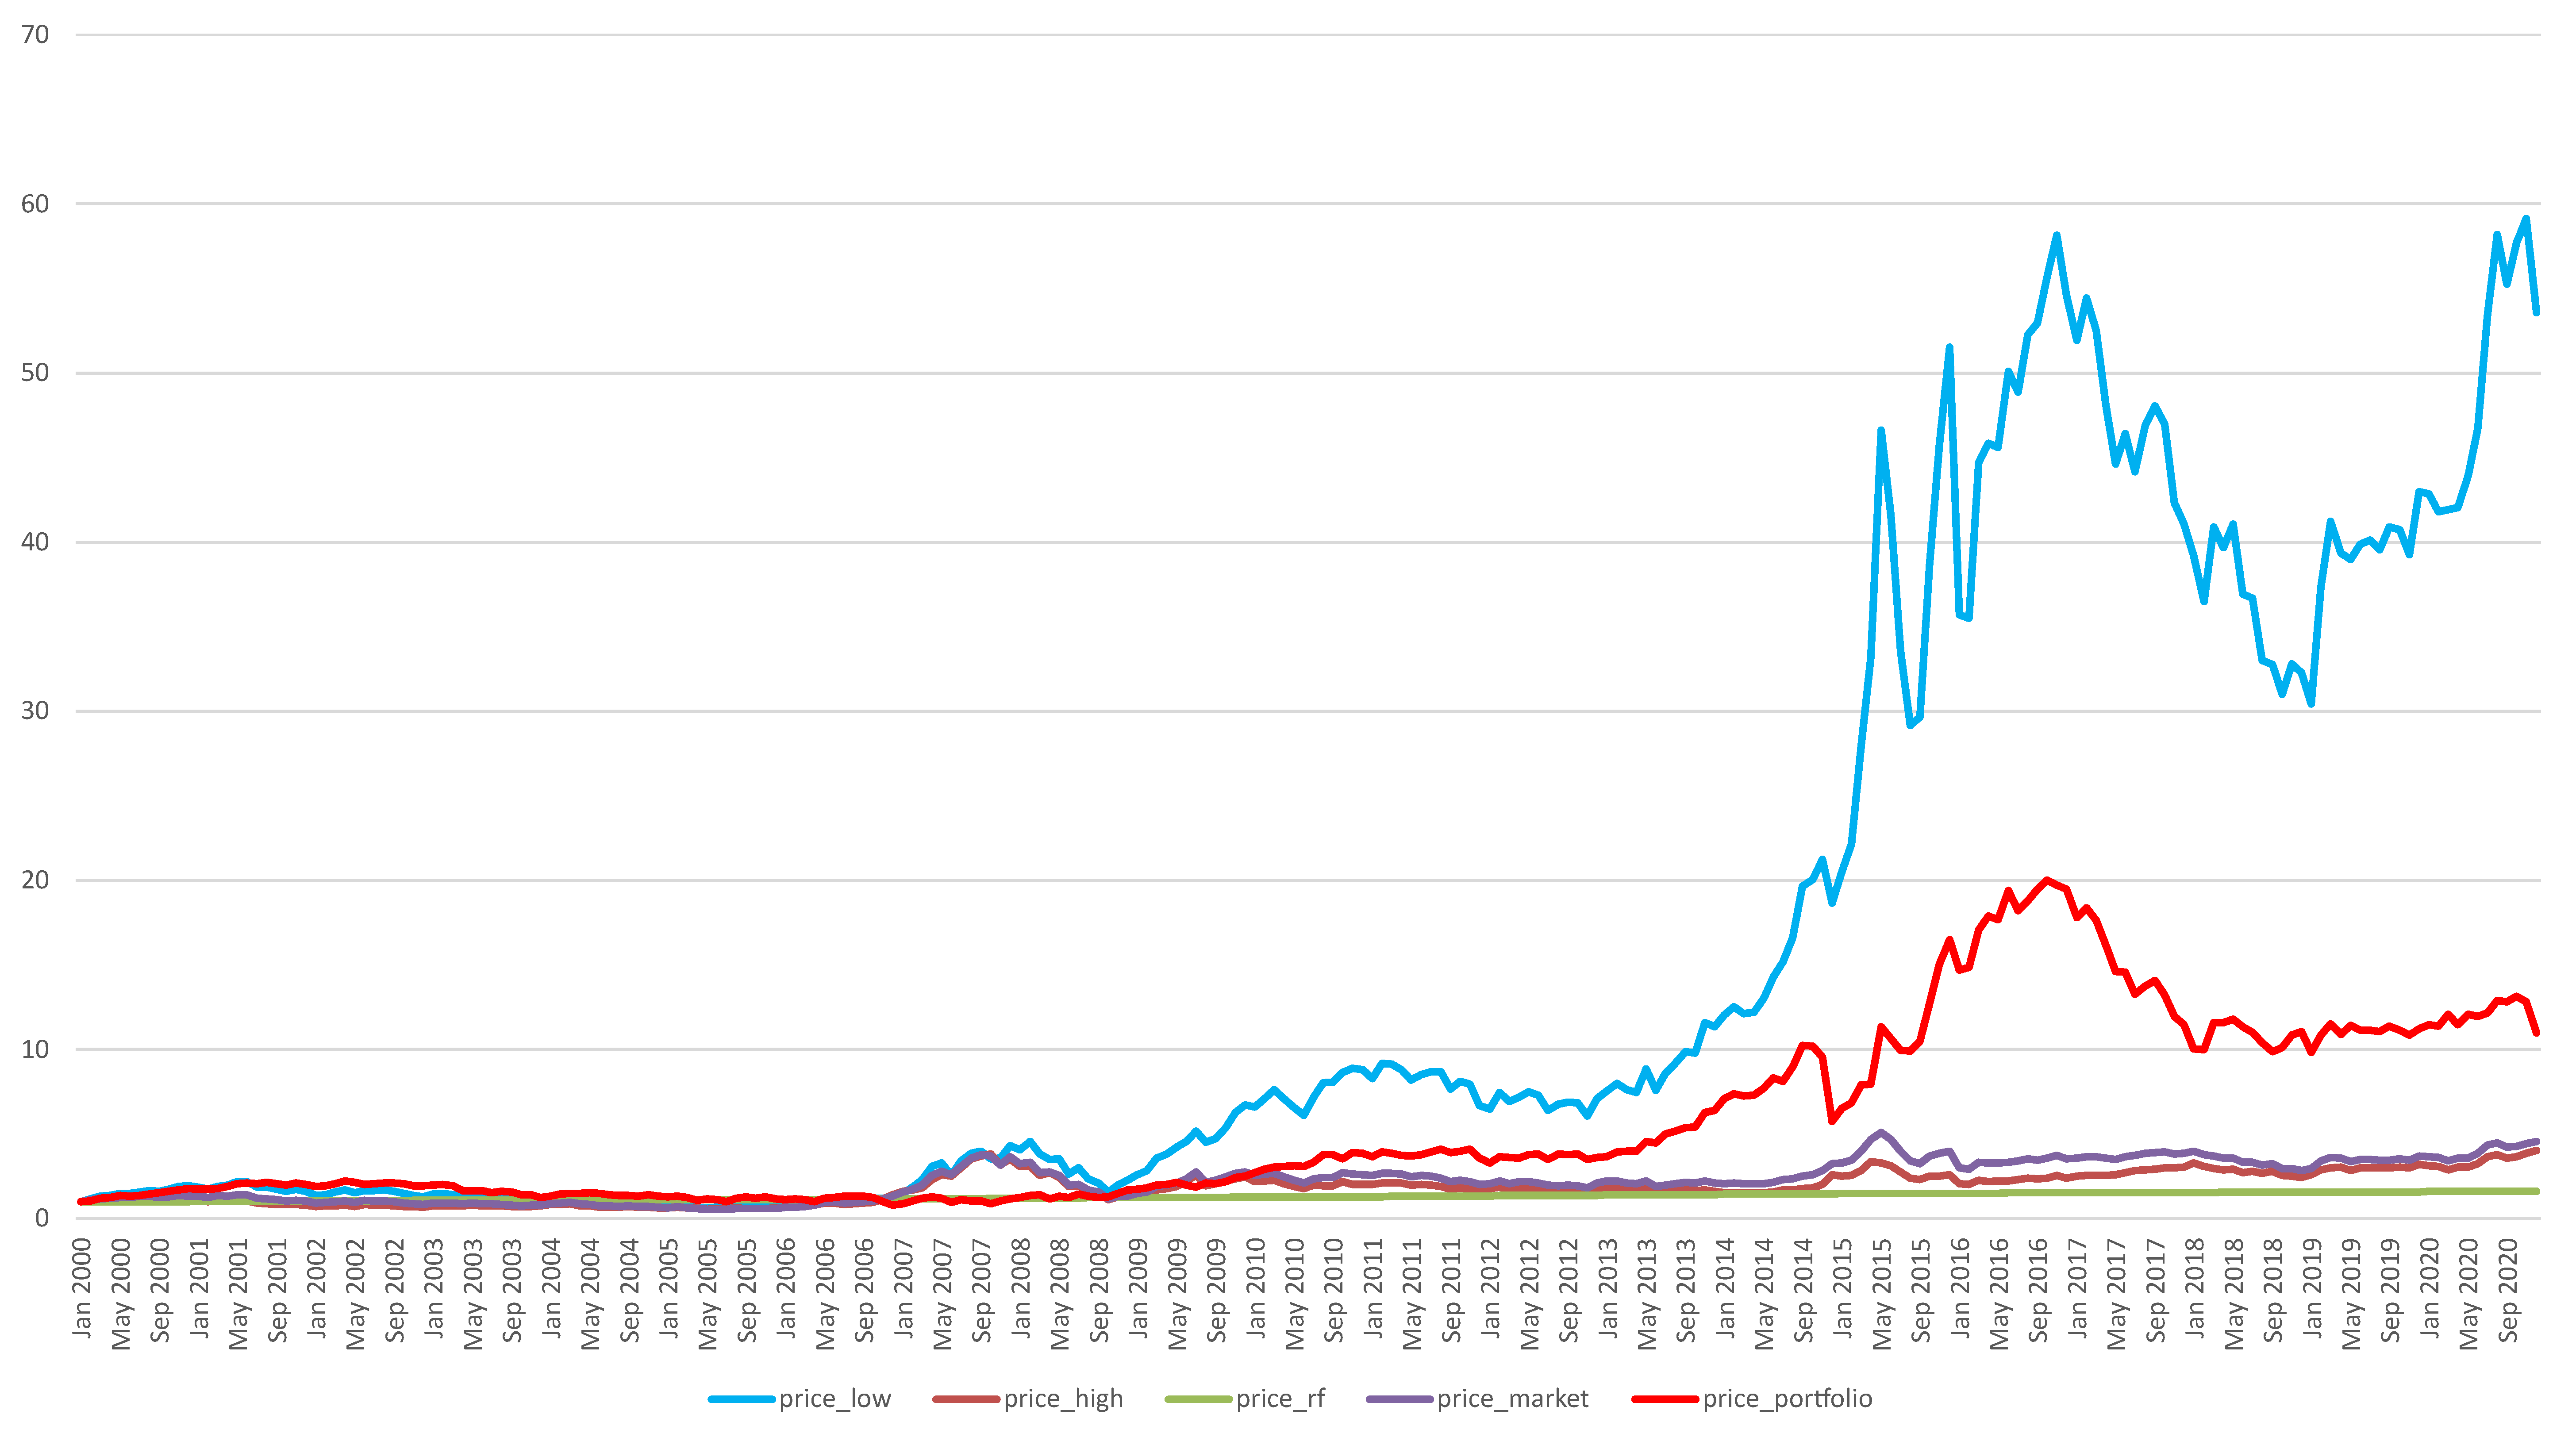
\includegraphics[width=\linewidth]{Files/size.pdf}
			
			\vspace{0.2cm}
			\footnotesize Size-sorted portfolios: the spread is strongest toward the small-stock end.
		\end{column}
		\begin{column}{0.49\textwidth}
			\centering
			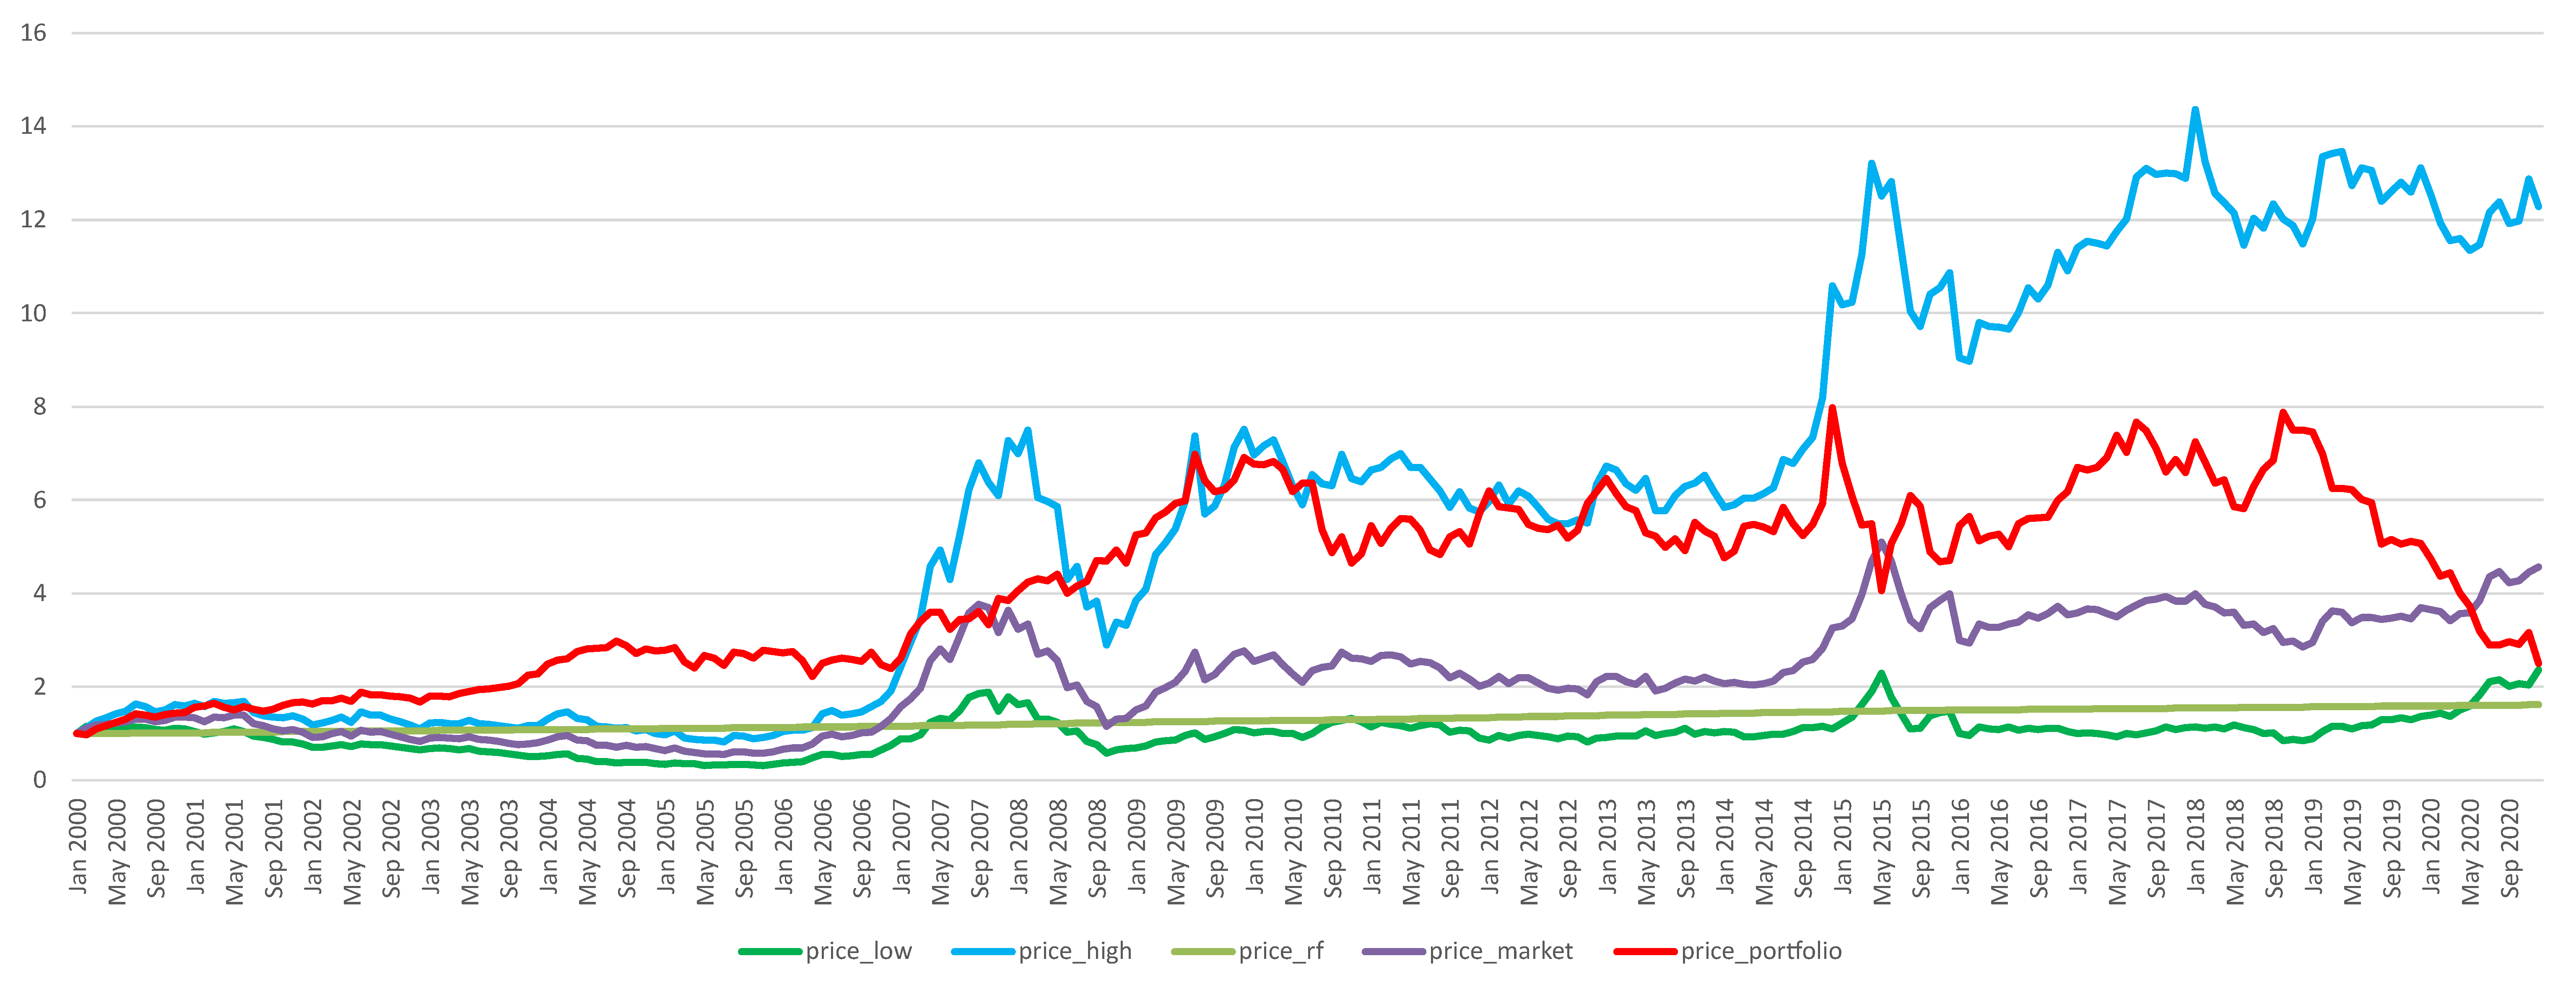
\includegraphics[width=\linewidth]{Files/bm.pdf}
			
			\vspace{0.2cm}
			\footnotesize B/M-sorted portfolios: value portfolios earn higher average returns than growth portfolios.
		\end{column}
	\end{columns}
\end{frame}

\begin{frame}{Momentum: The Premier Anomaly}
	\begin{itemize}
		\item \href{https://doi.org/10.1111/j.1540-6261.1993.tb04702.x}{\textcolor{blue}{Jegadeesh and Titman (1993)}} document that recent winners continue to outperform recent losers.
		\item Standard implementation: rank on past 12-month return with a \textbf{one-month skip}, then buy winners and short losers.
		\item \textbf{Why embarrassing?}
		\begin{itemize}
			\item Winners often look like growth stocks.
			\item Losers often look like value stocks.
			\item FF3 therefore predicts too much return for losers and too little for winners, making momentum alpha even larger.
		\end{itemize}
		\item \href{https://doi.org/10.1111/j.1540-6261.2008.01371.x}{\textcolor{blue}{Fama and French (2008)}} call momentum the \textbf{premier anomaly}.
	\end{itemize}
\end{frame}

\begin{frame}{Momentum Is Large on Average, but It Crashes}
	\begin{figure}
		\centering
		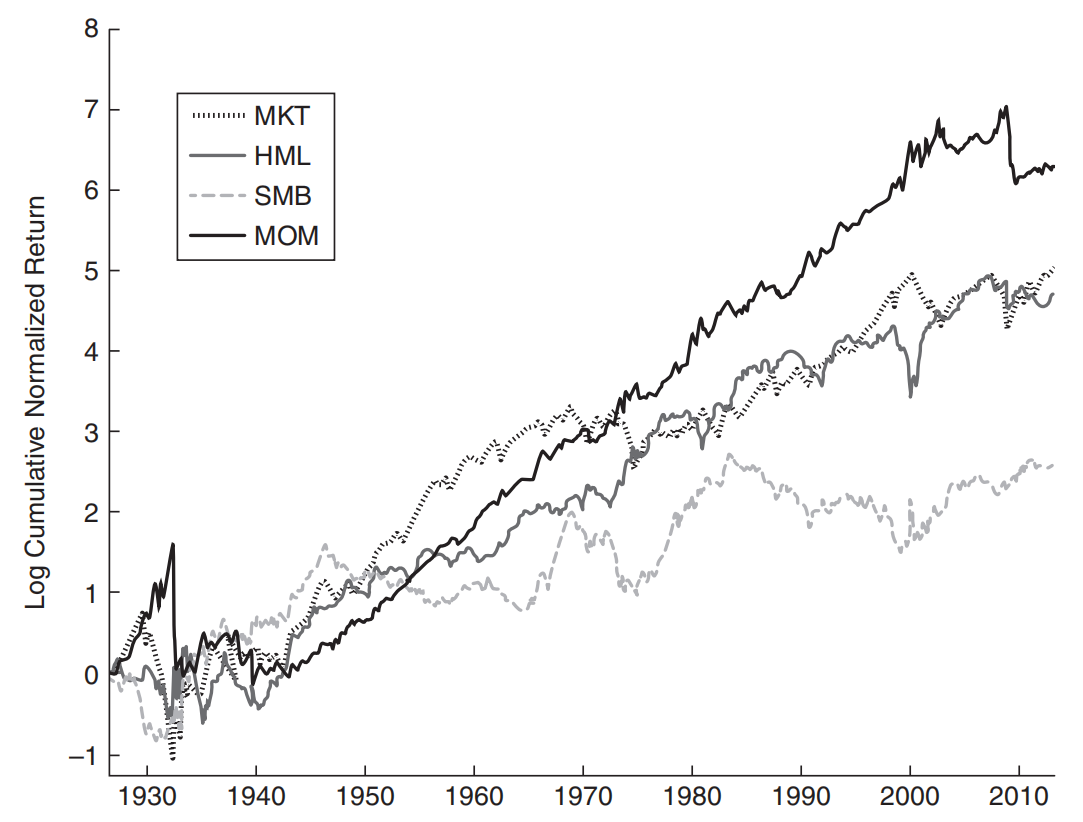
\includegraphics[width=0.73\linewidth]{Files/mom.png}
		\caption{Cumulative normalized factor returns, highlighting the large average momentum premium and occasional crash episodes.}
	\end{figure}
\end{frame}

\begin{frame}{Profitability and Investment}
	\begin{itemize}
		\item \textbf{Profitability}: \href{https://doi.org/10.1016/j.jfineco.2013.01.003}{\textcolor{blue}{Novy-Marx (2013)}} shows that more profitable firms earn higher returns.
		\item \textbf{Investment}: \href{https://doi.org/10.1111/j.1540-6261.2008.01370.x}{\textcolor{blue}{Cooper, Gulen, and Schill (2008)}} show that firms with high asset growth earn lower subsequent returns.
		\item These patterns are especially important because they connect directly to \textbf{production-based asset pricing}:
		\begin{itemize}
			\item high expected profitability $\Rightarrow$ high discount rate
			\item aggressive investment $\Rightarrow$ low cost of capital
		\end{itemize}
		\item They motivate \href{https://doi.org/10.1016/j.jfineco.2014.10.010}{\textcolor{blue}{FF5 (2015)}} and the \href{https://doi.org/10.1093/rfs/hhu068}{\textcolor{blue}{$q$-factor model}}.
	\end{itemize}
\end{frame}

\begin{frame}{Low-Risk, Idiosyncratic Volatility, and Liquidity}
	\begin{itemize}
		\item \textbf{Low-risk anomaly}: low-$\beta$ or low-volatility stocks often outperform high-$\beta$ stocks on a risk-adjusted basis.
		\item \textbf{Idiosyncratic volatility}: \href{https://doi.org/10.1111/j.1540-6261.2006.00836.x}{\textcolor{blue}{Ang, Hodrick, Xing, and Zhang (2006)}} document that high-IVOL stocks earn unusually low returns.
		\item \textbf{Liquidity}: illiquid stocks tend to earn higher average returns, consistent with \href{https://doi.org/10.1086/374184}{\textcolor{blue}{P\'astor and Stambaugh (2003)}} and related work.
		\item These anomalies are hard to place in a simple CAPM world:
		\begin{itemize}
			\item some look like \textbf{friction premia},
			\item some look like \textbf{lottery demand},
			\item some look like \textbf{delegated management constraints}.
		\end{itemize}
	\end{itemize}
\end{frame}

\begin{frame}{A Compact Map of Major Anomalies}
	\scriptsize
	\begin{table}
		\centering
		\resizebox{\linewidth}{!}{
			\begin{tabular}{llll}
				\toprule
				\textbf{Anomaly} & \textbf{Signal} & \textbf{Typical Spread} & \textbf{Later Factor Link} \\
				\midrule
				Size & Market equity & Small minus big $>$ 0 & SMB \\
				Value & Book-to-market & High B/M minus low B/M $>$ 0 & HML \\
				Momentum & Past 12-month return & Winners minus losers $>$ 0 & UMD / MOM \\
				Profitability & Gross profits / assets & Robust minus weak $>$ 0 & RMW / ROE \\
				Investment & Asset growth / I/A & Conservative minus aggressive $>$ 0 & CMA / I/A \\
				Low-risk & Beta or volatility & Low-risk minus high-risk $>$ 0 & BAB / low-vol \\
				Liquidity & Trading frictions & Illiquid minus liquid $>$ 0 & LIQ \\
				\bottomrule
			\end{tabular}
		}
	\end{table}

	\normalsize
	\textbf{Interpretive point:} once enough anomalies line up systematically, researchers naturally ask whether a \textbf{small set of factors} can span them.
\end{frame}

\section{Competing Explanations}

\begin{frame}{Risk-Based Interpretation}
	\textbf{The efficient-markets defense} is simple: an anomaly is just compensation for \textbf{missing risk}.

	\vspace{0.2cm}
	\begin{itemize}
		\item \textbf{ICAPM / APT logic}: multiple state variables, not just market beta, can price assets.
		\item \textbf{Value}: may proxy for distress or bad-times cash-flow sensitivity.
		\item \textbf{Profitability / Investment}: fit naturally with production-based models.
		\item \textbf{Momentum}: sometimes linked to crash risk or time-varying expected returns.
		\item \textbf{Low-risk}: often interpreted through leverage or funding constraints.
		\item Canonical reference: \href{https://doi.org/10.1016/j.jfineco.2013.10.005}{\textcolor{blue}{Frazzini and Pedersen (2014)}}.
	\end{itemize}

	\vspace{0.3cm}
	\textbf{Empirical implication}: if the risk story is correct, a well-designed factor model should drive anomaly alphas toward zero.
\end{frame}

\begin{frame}{Behavioral and Mispricing Interpretation}
	\begin{itemize}
		\item \textbf{Underreaction}: prices adjust too slowly to news.
		\item \textbf{Overreaction}: investors extrapolate too much from recent performance.
		\item \textbf{Limited attention}: complex signals enter prices only gradually.
		\item \textbf{Sentiment}: speculative demand overprices hard-to-arbitrage assets.
	\end{itemize}

	\vspace{0.2cm}
	\textbf{Canonical references}
	\begin{itemize}
		\item \href{https://doi.org/10.1111/j.1540-6261.1985.tb05004.x}{\textcolor{blue}{De Bondt and Thaler (1985)}}: long-run reversal and overreaction.
		\item \href{https://doi.org/10.1016/S0304-405X(98)00027-0}{\textcolor{blue}{Barberis, Shleifer, and Vishny (1998)}}: conservatism and representativeness.
		\item \href{https://doi.org/10.1111/0022-1082.00077}{\textcolor{blue}{Daniel, Hirshleifer, and Subrahmanyam (1998)}}: overconfidence and self-attribution.
		\item \href{https://doi.org/10.1111/j.1540-6261.2006.00885.x}{\textcolor{blue}{Baker and Wurgler (2006)}}: sentiment.
	\end{itemize}

	\textbf{Prediction}: anomalies should be strongest where arbitrage is hard and investor sophistication is low.
\end{frame}

\begin{frame}{Why Does Mispricing Persist?}
	\textbf{Limits to arbitrage} prevent smart money from instantly eliminating anomalies.

	\begin{itemize}
		\item \textbf{Fundamental risk}: mispricing can widen before it closes.
		\item \textbf{Noise-trader risk}: sentiment creates painful mark-to-market losses.
		\item \textbf{Implementation frictions}: short-sale constraints, borrow fees, and trading costs.
		\item \textbf{Delegated management}: benchmark constraints and career concerns reduce aggressive arbitrage.
	\end{itemize}

	\vspace{0.2cm}
	\textbf{Classic reference}: \href{https://doi.org/10.1111/j.1540-6261.1997.tb03807.x}{\textcolor{blue}{Shleifer and Vishny (1997)}}.

	\vspace{0.3cm}
	\begin{block}{Practical implication}
		Even if an anomaly is genuine mispricing, it does not follow that it is easy to monetize in institutional size.
	\end{block}
\end{frame}

\begin{frame}{Characteristics vs. Factors}
	\begin{itemize}
		\item An empirical regularity can show up first as a \textbf{characteristic} (for example, book-to-market) and only later be turned into a \textbf{factor portfolio} (HML).
		\item A factor is a \textbf{summary portfolio}; it is \textit{not} by itself proof of a deep structural state variable.
		\item This creates a core doctoral-level debate:
		\begin{enumerate}
			\item Do \textbf{covariances} with factors explain expected returns?
			\item Or do \textbf{characteristics} contain information beyond covariances?
		\end{enumerate}
		\item In practice, modern empirical asset pricing uses both views:
		\begin{itemize}
			\item characteristics discover anomalies,
			\item factor models organize and price them.
		\end{itemize}
	\end{itemize}
\end{frame}

\section{What Survives Scrutiny}

\begin{frame}{Replication Crisis and Multiple Testing}
	\begin{itemize}
		\item \href{https://doi.org/10.1093/rfs/hhv059}{\textcolor{blue}{Harvey, Liu, and Zhu (2016)}} argue that the literature faces a serious \textbf{multiple testing} problem.
		\item Practical takeaway: for a \textbf{new} anomaly, a $t$-statistic near 2 is usually not enough; a hurdle closer to \textbf{3.0} is more defensible.
		\item \href{https://doi.org/10.1093/rfs/hhy131}{\textcolor{blue}{Hou et al. (2020)}} show that many published anomalies weaken under a common replication protocol.
		\item Recent synthesis work suggests that only a \textbf{small core set} of characteristics remains dominant once redundancy is addressed.
	\end{itemize}

	\vspace{0.3cm}
	\begin{beamercolorbox}[sep=0.4em,wd=\linewidth,rounded=true,shadow=true]{postit}
		\textbf{Lesson:} modern anomaly research is as much about \textbf{selection discipline} as about discovery itself.
	\end{beamercolorbox}
\end{frame}

\begin{frame}{Statistical Significance Is Not Economic Significance}
	\begin{itemize}
		\item \textbf{Turnover}: fast signals can look strong gross but disappear net of costs.
		\item \textbf{Capacity}: many spreads are strongest in stocks that cannot absorb large capital.
		\item \textbf{Shorting}: negative legs are often the hard part of implementation.
		\item \textbf{Publication decay}: \href{https://doi.org/10.1111/jofi.12365}{\textcolor{blue}{McLean and Pontiff (2016)}} show post-publication return decay.
	\end{itemize}

	\vspace{0.3cm}
	\textbf{Hence a serious empirical paper should report}
	\begin{itemize}
		\item gross and net returns,
		\item long leg, short leg, and long-short separately,
		\item turnover and holding horizon,
		\item robustness excluding microcaps.
	\end{itemize}
\end{frame}

\begin{frame}{External Validity: Why China Matters}
	\begin{itemize}
		\item International evidence separates \textbf{universal mechanisms} from \textbf{market-structure artifacts}.
		\item In China, anomalies are often shaped by:
		\begin{itemize}
			\item dominant retail participation,
			\item short-sale frictions,
			\item shell value and listing option value,
			\item policy shocks and changing market institutions.
		\end{itemize}
		\item A useful example: momentum is historically much weaker in A-shares than in many developed markets, while value and turnover-related effects are highly market-structure dependent.
		\item For doctoral work, China is not just ``another sample''; it is a \textbf{laboratory for mechanism testing}.
	\end{itemize}
\end{frame}

\begin{frame}{Recent Frontier I: Alternative Data in the Cross-Section}
	\scriptsize
	\begin{table}
		\centering
		\resizebox{\linewidth}{!}{
			\begin{tabular}{p{2.9cm}p{3.6cm}p{4.6cm}}
				\toprule
				\textbf{Alternative Data} & \textbf{Recent Paper} & \textbf{Main Cross-Sectional Insight} \\
				\midrule
				Earnings-call climate text & \href{https://doi.org/10.1093/rfs/hhad094}{\textcolor{blue}{Li, Shan, Tang, and Yao (2024)}} & Transition climate risk extracted from call transcripts is priced; firms that do not respond proactively trade at a discount. \\
				Media tone disagreement & \href{https://doi.org/10.1016/j.iref.2025.104751}{\textcolor{blue}{Media tone disagreement in China (2025)}} & Disagreement in media coverage predicts future returns, especially when short selling is constrained and sentiment is weak. \\
				Employee review platforms & \href{https://doi.org/10.1016/j.pacfin.2025.102847}{\textcolor{blue}{Bae and Ha (2025)}} & Job-platform satisfaction scores predict about 1.11\% per month winner-minus-loser spreads in Korea. \\
				Patent inventor networks & \href{https://doi.org/10.1016/j.ribaf.2025.103004}{\textcolor{blue}{Bae, Kim, and Kwon (2025)}} & More integrated inventor networks predict higher long-run returns through innovation quality and key-talent risk. \\
				\bottomrule
			\end{tabular}
		}
	\end{table}

	\normalsize
	\textbf{Pattern:} the most useful alternative data are usually proxies for \textbf{intangible capital}, \textbf{beliefs}, or \textbf{non-accounting risk exposures}.
\end{frame}

\begin{frame}{Recent Frontier II: What Is New in 2024--2026?}
	\begin{itemize}
		\item \href{https://doi.org/10.1016/j.jfineco.2024.103952}{\textcolor{blue}{He, Su, and Yu (2024)}}: subjective macroeconomic perceptions help \textbf{time} many anomalies; optimism strengthens quality and low-risk but weakens value and investment.
		\item \href{https://doi.org/10.1093/rapstu/raaf001}{\textcolor{blue}{M\"uller and Schmickler (2025)}}: anomaly payoffs are not additively separable; double sorts uncover many economically large interactions.
		\item \href{https://www.nber.org/papers/w32767}{\textcolor{blue}{Hirshleifer and Ma (2025 revision)}} show that EDGAR and XBRL shrink \textbf{accounting-based anomalies}, directly linking market efficiency to information technology.
		\item \href{https://www.nber.org/papers/w34009}{\textcolor{blue}{Chernov, Dahlquist, and Lochstoer (July 2025)}} argue that many characteristic factors contain large \textbf{unpriced components}; hedging them can sharply raise Sharpe ratios.
		\item \href{https://doi.org/10.1016/j.pacfin.2026.103109}{\textcolor{blue}{Abnormal analyst coverage in China (2026)}}: unusual analyst coverage predicts later ROA surprises and stock returns.
	\end{itemize}
\end{frame}

\section{Bridge to Factors}

\begin{frame}{From Anomalies to Factor Models}
	\small
	\begin{table}
		\centering
		\resizebox{\linewidth}{!}{
			\begin{tabular}{lll}
				\toprule
				\textbf{Empirical Failure} & \textbf{Factor Response} & \textbf{Benchmark Model} \\
				\midrule
				CAPM misses size and value & Add SMB and HML & FF3 \\
				FF3 misses momentum & Add UMD / MOM & Carhart 4-factor \\
				FF3 misses profitability and investment & Add RMW and CMA & FF5 \\
				Value/investment linked to firm production & ROE and I/A factors & $q$-factor \\
				Low-risk and liquidity spreads remain & Add BAB / LIQ / others & Extended models \\
				\bottomrule
			\end{tabular}
		}
	\end{table}

	\normalsize
	\begin{itemize}
		\item Factor models are the profession's attempt to \textbf{compress many anomalies into a parsimonious SDF}.
		\item The next lecture asks a harder question: \textbf{which factors deserve benchmark status?}
	\end{itemize}
\end{frame}

\begin{frame}{What Counts as a Successful Factor Model?}
	\begin{itemize}
		\item \textbf{Small alphas}: anomaly spreads should be close to zero after controlling for the factors.
		\item \textbf{Good cross-sectional fit}: high-$\beta$ assets to the factor should earn high average returns if the factor is truly priced.
		\item \textbf{Economic interpretation}: the factor should connect to risk, production, intermediation, or a disciplined mispricing story.
		\item \textbf{Robustness}: results should survive alternative samples, weights, and tradability filters.
	\end{itemize}

	\vspace{0.3cm}
	\textbf{Evaluation toolkit}
	\begin{itemize}
		\item Time-series alphas and the GRS test
		\item Fama-MacBeth risk premia
		\item Hansen-Jagannathan distance / maximum Sharpe ratio
	\end{itemize}
\end{frame}

\begin{frame}{Suggested Readings for a PhD Seminar}
	\begin{itemize}
		\item \href{https://doi.org/10.1111/j.1540-6261.1992.tb04398.x}{\textcolor{blue}{Fama and French (1992)}}: cross-section of expected stock returns.
		\item \href{https://doi.org/10.1016/0304-405X(93)90023-5}{\textcolor{blue}{Fama and French (1993)}}: the FF3 benchmark.
		\item \href{https://doi.org/10.1111/j.1540-6261.1993.tb04702.x}{\textcolor{blue}{Jegadeesh and Titman (1993)}}: momentum.
		\item \href{https://doi.org/10.1111/j.1540-6261.2008.01371.x}{\textcolor{blue}{Fama and French (2008)}}: dissecting anomalies.
		\item \href{https://doi.org/10.1093/rfs/hhu068}{\textcolor{blue}{Hou, Xue, and Zhang (2015)}}: digesting anomalies via investment.
		\item \href{https://doi.org/10.1093/rfs/hhv059}{\textcolor{blue}{Harvey, Liu, and Zhu (2016)}}: multiple testing.
		\item \href{https://doi.org/10.1093/rfs/hhy131}{\textcolor{blue}{Hou, Xue, and Zhang (2020)}}: replication.
		\item \href{https://doi.org/10.1287/mnsc.2023.4904}{\textcolor{blue}{Li, Liu, Liu, and Wei (2024)}}: Chinese A-share replication.
	\end{itemize}
\end{frame}

\begin{frame}{Takeaways}
	\begin{enumerate}
		\item An anomaly is an \textbf{alpha relative to a benchmark}, not a model-free fact.
		\item The major anomalies are sufficiently systematic that they force us beyond CAPM.
		\item The central disputes are \textbf{risk vs. mispricing} and \textbf{discovery vs. data mining}.
		\item Good anomaly research requires careful design, strong inference, and implementation realism.
		\item Multi-factor models are best understood as \textbf{organizational responses} to the anomaly evidence.
	\end{enumerate}

	\vspace{0.4cm}
	\centering
	\textbf{Next lecture:} From anomalies to benchmark factor models: FF3, Carhart, FF5, and beyond.
\end{frame}

\end{document}
